\section{ELO Algorithm}


ELO - The algorithm made famous by Facebook \& depicted in the movie \textit{Social
Network}

\begin{figure}[h]
\centering
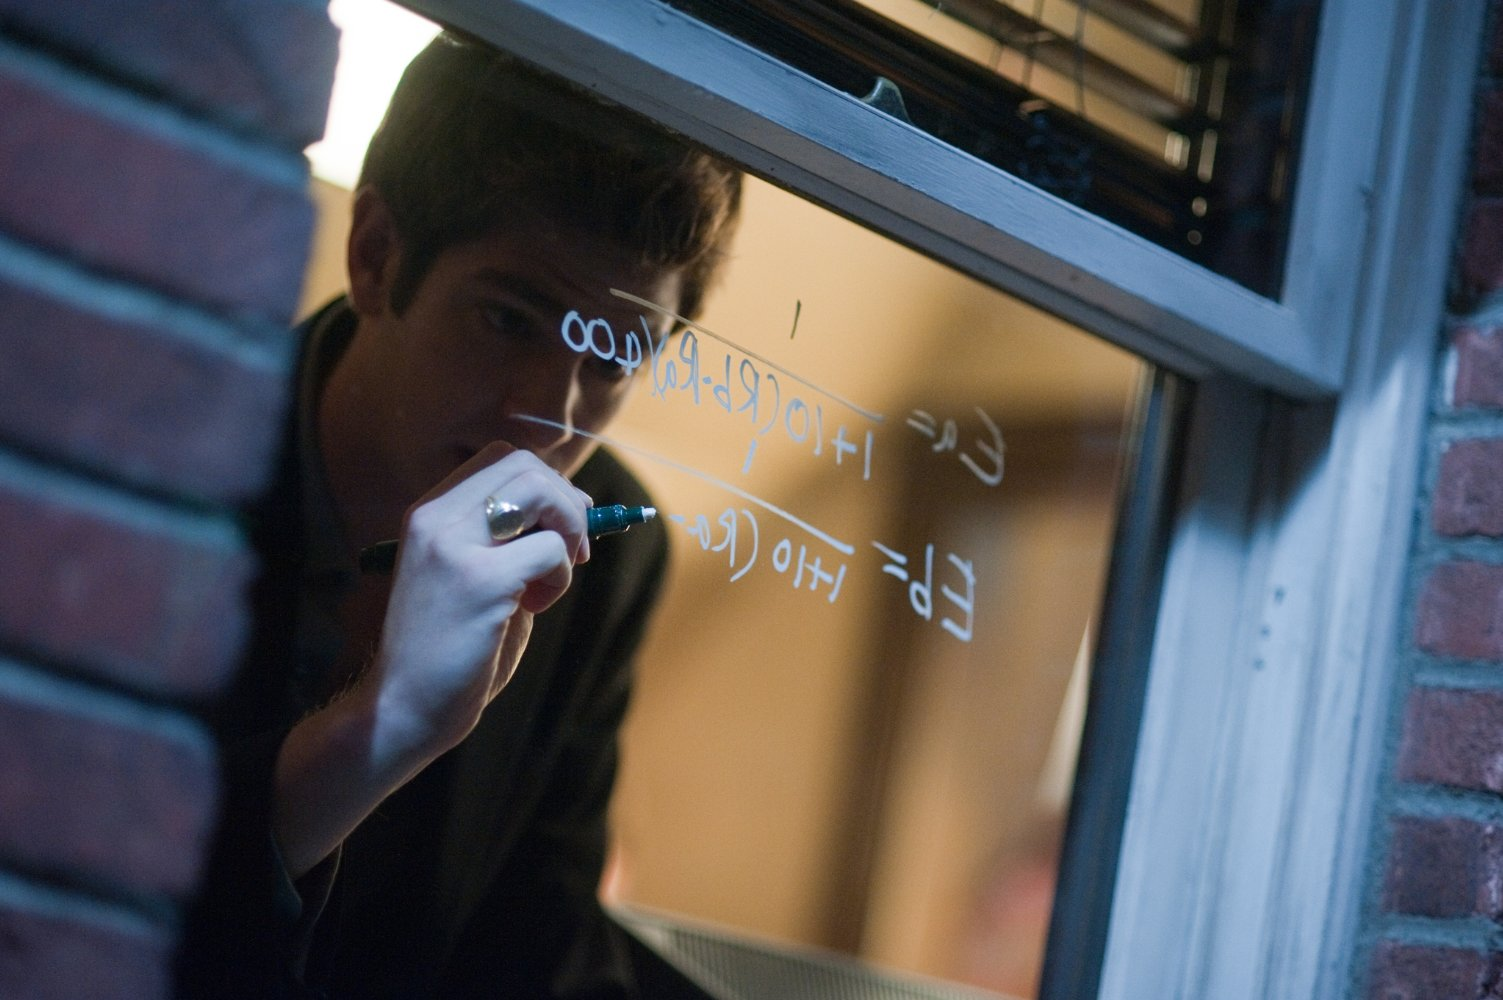
\includegraphics[width=15cm,height=8cm,scale = 0.5]{facebook}
\end{figure}

\begin{itemize}
  \item Basic Chess Algorithm proposed by Arpad Emrick Elo:

\[ _{n}R_{i} = _{o}R_{i} + K(S_{ij} - \mu_{ij}) \]

Where 
\[ \mu_{ij} = \frac{1}{1+10^{(_{o}R_{i} - _{o}R_{j})/400}} \] is the expected
result, K factor is adjusted for each domain. For Chess, K = 10; for soccer it 
varies from 20 to 60. $S_{ij} = 1$ or $1/2$ or $0$.


  \item  ELO Algorithm adjusted to basketball game:


For chess game, no score needed to be considered except Win, Lose or Draw;
but ball games have scores that need to be accommodated.


In this project, ELO rating for each team is updated per game using following
formula:

\[ _{n}R_{i} = _{o}R_{i} + K*M_{ov}(S_{ij} - \mu_{ij}) \]


where 
\[ M_{ov} = \frac{(abs(PD) + 3)^{0.8}}{7.5 + 0.006*(elo\_diff)} \]


In this algorithm, K factor takes value 20. 
\[ elo\_diff = (abs(R_{i} - R_{j})+100*home\_win)*won\_underdog \]


where $home\_win = 1$ if the home team won the game, 0 otherwise. $won\_underdog$ 
takes value of 1 if the team got expected outcome as suggested by the ELO rank, -1 otherwise.

\end{itemize}

 
By using the ELO rating system, we can also calculate one team's probability
of winning:

\[ Pr(A) = \frac{1}{10 ^{-elo\_diff/400}+1} \]

But in our model, we only use this as one factor.


